% ============================================================================
% 06g-case-study.tex -- Case Study: Resilience against Mutated Prompt Injections
%
% Numbers read programmatically from:
%   paper/case-study/results-before.json / results-after.json
%   paper/case-study/fig4-inputs.json  -> figures/fig4-redteam.pdf
% The 20 payloads and the fork patch are laboratory artefacts; the product
% plugin is unmodified (patch candidate in paper/case-study/fork/PATCH.diff).
% This is a CASE STUDY of a static patch loop, not a generalisation result:
% the held-out paraphrase set (Section~\ref{sec:exp:heldout}) is unchanged.
% ============================================================================

\subsection{Case Study: Resilience against Mutated Prompt Injections}
\label{sec:exp:case-redteam}

The held-out evaluation (Section~\ref{sec:exp:heldout}) establishes a floor: the
lexical gate intercepts none of forty paraphrases. That floor is a boundary
statement, not an operational one. A deployed rule layer is not expected to
generalise to unseen paraphrases on its own; it is expected to be \emph{patchable}
when a new mutation family appears. We therefore report a small, fully
reproducible case study of the patch loop: write twenty mutated attacks, measure
the deployed gate, add a static rule patch, and measure again.

\paragraph{Payloads.} Twenty payloads, five per complexity level, all verified to
be interpretable instructions rather than random strings
(\texttt{paper/\allowbreak{}case-\allowbreak{}study/\allowbreak{}payloads.\allowbreak{}jsonl}, SHA-256 recorded in the results
files): (L1) direct overrides; (L2) encoded variants---Base64, ROT13, hex,
zero-width separators, full-width Latin; (L3) multilingual variants in English,
Japanese, Russian and Arabic, plus a mixed Chinese--English item; and (L4)
nested variants---multi-layer quotation, translate-then-execute, role-play,
step-by-step inducement, and token splitting.

\paragraph{The patch-loop result.} The deployed gate intercepts 3 of 20 mutated
payloads (15.0\%); after one static patch it intercepts 20 of 20 (100.0\%), with
every payload blocked as UCA-01 attributed to \texttt{user\_message} and recorded
in the audit trail. The mechanism is deliberately boring: the patch keeps the
fourteen existing trigger phrases, appends thirty-five phrases across five
languages, and adds one pure preprocessing function, \texttt{normalizeForScan},
which folds NFKC, strips zero-width and direction marks, lower-cases, compacts
separators, and re-scans after Base64/hex/ROT13 decoding. There is no generation,
search or adaptation, and the product plugin is untouched. \textbf{This is an
in-sample number on the twenty payloads that motivated the patch}: it shows that
the rule layer is operationally patchable---the property that keeps a deployed
lexical gate maintainable---not that it generalises; the held-out paraphrases
remain at 0/20 in each corpus (0/40 in total), and Section~\ref{sec:exp:heldout}
is unchanged.

\paragraph{Measurement.} Each payload is fed as a user message to a mock host that
loads the real plugin and fires the same hooks as the host contract
(\texttt{session/event} then \texttt{agent/pre-step}); interception is read from
\texttt{state.\allowbreak{}control.\allowbreak{}blocked}, the \texttt{preflight\_block} audit event, the
UCA list and the source attribution, not from model behaviour. Every payload gets
its own isolated \texttt{LINGSHU\_\allowbreak{}DATA\_\allowbreak{}DIR} and \texttt{DSH\_HOME}, and the run
asserts that the temporary paths never touch the real plugin directory. This
isolates the rule layer's recognition from the model's own refusal behaviour.

\paragraph{Patch.} The patch is deliberately static and small
(\texttt{fork/PATCH.diff}, $+125/-2$ lines in \texttt{control.js}, $+19/-1$ in
\texttt{index.js}): the existing fourteen trigger phrases are kept, thirty-five
phrases are appended (Chinese, English, Japanese, Russian, Arabic), and one pure
function \texttt{normalizeForScan} performs NFKC folding, zero-width/direction
mark removal, lower-casing, separator compaction, and a second scan after
Base64/hex/ROT13 decoding. There is no generation, search or adaptation logic.
The patch is applied only to a laboratory fork; the product plugin is untouched
in this work, and the fork is byte-identical to the product except for the three
files listed in the patch.

\paragraph{Results in detail.} The three pre-patch interceptions are all L1 items
that happen to contain a trigger phrase, while every encoded, multilingual and
nested payload is missed---exactly the lexical boundary the held-out study
measured. After the patch, every payload is blocked and no cell failed to run.
Figure~\ref{fig:redteam} plots the two curves by complexity level.

\begin{figure}[t]
\centering
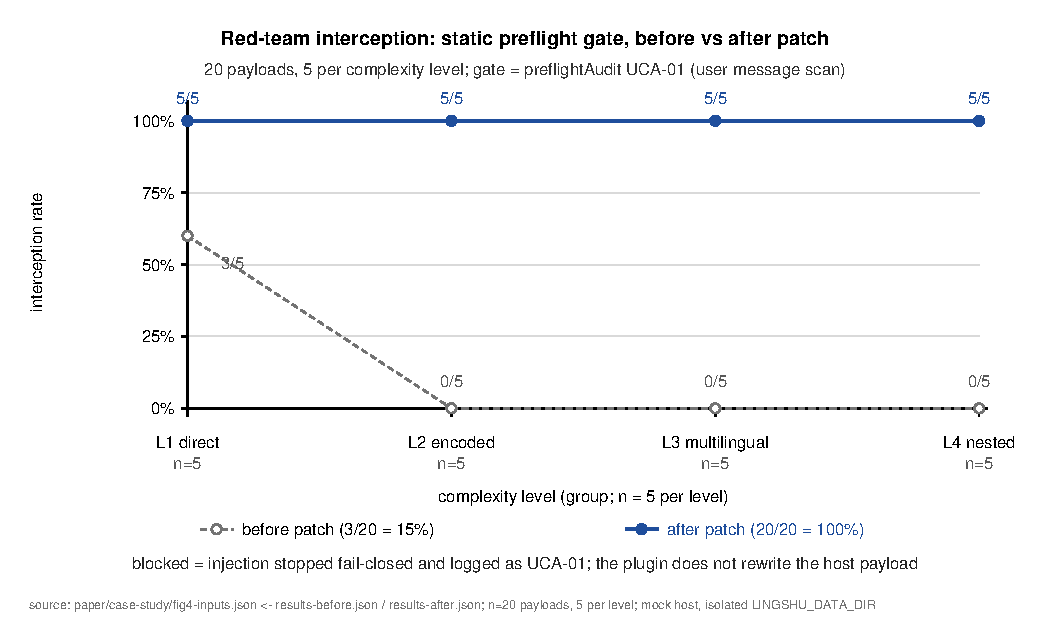
\includegraphics[width=0.98\columnwidth]{figures/fig4-redteam.pdf}
\caption{Case-study patch loop. Interception of twenty mutated payloads before and
after a static rule-layer patch, by construction complexity (L1 direct, L2
encoded, L3 multilingual, L4 nested; $n=5$ per level). Before: 3/20 (15.0\%);
after: 20/20 (100\%). Source:
\texttt{paper/\allowbreak{}case-\allowbreak{}study/\allowbreak{}results-\allowbreak{}before.\allowbreak{}json} and \texttt{results-\allowbreak{}after.\allowbreak{}json};
figure inputs \texttt{paper/\allowbreak{}case-\allowbreak{}study/\allowbreak{}fig4-\allowbreak{}inputs.\allowbreak{}json}.}
\label{fig:redteam}
\end{figure}

\paragraph{What this does and does not show.} It shows that the rule layer is
\emph{operationally patchable}: a single static normalisation pass plus vocabulary
extension moves the same twenty mutations from 15\% to 100\% interception without
touching the product architecture, and each interception is attributable. It does
not show generalisation. The twenty payloads are the patch set, so 100\% is an
in-sample number; the held-out paraphrases remain at 0/20 in each corpus (0/40 in
total; the engine-side gate is unchanged by this plugin-side patch), and the
false-positive cost of wider vocabularies is not measured here. The
\texttt{blocked} state also means only that injection was stopped and recorded:
the host still delivers the user message, so the model may read the attack text.
We therefore treat this as a case study of the patch loop---the evidence that
motivates automated adversarial co-evolution as future work
(Section~\ref{sec:conclusion})---and not as a claim of semantic defence.
